\chapter{User Study Results - Supplementary Data}
\label{appendix:results}

This appendix provides comprehensive detailed data and statistical analyses supporting Chapter~\ref{chapter:results}. The structure mirrors the main results chapter organization, with each section containing complete datasets, statistical test results, and additional analyses referenced in the main text.

\textbf{Statistical Approach:} Within-subjects design with 8 dyads (16 participants), 4 collaboration variants, Latin square randomization. Friedman tests for repeated measures comparisons, Wilcoxon signed-rank for post-hoc analysis, Spearman correlations for relationships between variables.

\subsection{Participant ID Reference}

For data privacy, all participants are identified using anonymized codes throughout this appendix. The following table provides the mapping between participant numbers (0-15; as used in the main text) and their corresponding anonymised identifiers:

\begin{table}[H]
\centering
\caption{Participant ID Mapping Reference}
\label{tab:participant_id_mapping}
\begin{tabular}{cl}
\toprule
\textbf{No.} & \textbf{Participant ID} \\
\midrule
0 & 6m7xtdFy \\
1 & OYYOwkG2 \\
2 & Oa3Qww1v \\
3 & SAKl2Kyg \\
4 & WzyEiaaj \\
5 & YeUp7E4D \\
6 & dckk6p6S \\
7 & iB6kR2uo \\
8 & iN9X5S4Q \\
9 & j7hHkgiC \\
10 & jFYQhuSp \\
11 & kDp3Cy37 \\
12 & kHxWHBLy \\
13 & uTSV9lZx \\
14 & wocE408P \\
15 & zIDJJG4M \\
\bottomrule
\end{tabular}
\end{table}

% ============================================================================
\section{Study Overview and Participant Characteristics}
\label{appendix:study_overview}
% ============================================================================

\subsection{Study Design Summary}
\label{appendix:participants}

\begin{table}[H]
\centering
\caption{Complete Participant Demographics and Baseline Characteristics (N=16)}
\label{tab:demographics_appendix}
\begin{tabular}{lc}
\toprule
\textbf{Characteristic} & \textbf{Value} \\
\midrule
\textbf{Demographics} & \\
Age (years, mean ± SD) & 24.81 ± 2.17 \\
Age range & 22-29 years \\
Gender (Male/Female) & 10/6 (62.5\%/37.5\%) \\
Primary Language (German/Other) & 13/3 (81.3\%/18.7\%) \\
\midrule
\textbf{AR/VR Experience} & \\
None & 3 (18.8\%) \\
Limited & 11 (68.8\%) \\
Extensive & 2 (12.5\%) \\
\midrule
\textbf{Big Five Personality Traits} & \\
Openness & 3.56 ± 0.52 \\
Conscientiousness & 3.78 ± 0.42 \\
Extraversion & 3.59 ± 0.57 \\
Agreeableness & 3.94 ± 0.41 \\
Neuroticism & 2.31 ± 0.48 \\
\midrule
\textbf{Baseline Measures} & \\
Partner familiarity ("very well") & 9 (56.3\%) \\
Confidence in own performance (positive) & 13 (81.3\%) \\
Confidence in partner performance (positive) & 13 (81.3\%) \\
\bottomrule
\end{tabular}
\end{table}

% ============================================================================
\section{Task Performance Analysis - Detailed Results}
\label{appendix:completion_time_results}
% ============================================================================

\subsection{Complete Session-by-Session Performance Data}

\begin{longtable}{clllrr}
\caption{Complete Task Performance Dataset - All 32 Sessions}
\label{tab:all_completion_times} \\
\toprule
\textbf{Run} & \textbf{Dyad} & \textbf{Variant} & \textbf{Env} & \textbf{Pos} & \textbf{Time (min)} \\
\midrule
\endfirsthead
\multicolumn{6}{c}{\textit{(Continued from previous page)}} \\
\toprule
\textbf{Run} & \textbf{Dyad} & \textbf{Variant} & \textbf{Env} & \textbf{Pos} & \textbf{Time (min)} \\
\midrule
\endhead
\midrule
\multicolumn{6}{c}{\textit{(Continued on next page)}} \\
\endfoot
\bottomrule
\endlastfoot
1 & SAKl2Kyg-jFYQhuSp & Open Ended & 0 & 0 & 9.72 \\
2 & SAKl2Kyg-jFYQhuSp & Timed & 1 & 1 & 4.58 \\
3 & SAKl2Kyg-jFYQhuSp & Silent & 3 & 2 & 6.65 \\
4 & SAKl2Kyg-jFYQhuSp & Roleplay & 2 & 3 & 29.52 \\
5 & 6m7xtdFy-kHxWHBLy & Timed & 1 & 0 & 11.00 \\
6 & 6m7xtdFy-kHxWHBLy & Roleplay & 3 & 1 & 13.17 \\
7 & 6m7xtdFy-kHxWHBLy & Open Ended & 2 & 2 & 8.28 \\
8 & 6m7xtdFy-kHxWHBLy & Silent & 0 & 3 & 4.40 \\
9 & YeUp7E4D-WzyEiaaj & Silent & 3 & 0 & 8.27 \\
10 & YeUp7E4D-WzyEiaaj & Open Ended & 2 & 1 & 2.87 \\
11 & YeUp7E4D-WzyEiaaj & Roleplay & 0 & 2 & 3.87 \\
12 & YeUp7E4D-WzyEiaaj & Timed & 1 & 3 & 2.28 \\
13 & OYYOwkG2-dckk6p6S & Roleplay & 2 & 0 & 14.55 \\
14 & OYYOwkG2-dckk6p6S & Silent & 0 & 1 & 3.23 \\
15 & OYYOwkG2-dckk6p6S & Timed & 1 & 2 & 1.55 \\
16 & OYYOwkG2-dckk6p6S & Open Ended & 3 & 3 & 3.87 \\
17 & kDp3Cy37-wocE408P & Open Ended & 1 & 0 & 11.58 \\
18 & kDp3Cy37-wocE408P & Timed & 3 & 1 & 1.92 \\
19 & kDp3Cy37-wocE408P & Silent & 2 & 2 & 2.92 \\
20 & kDp3Cy37-wocE408P & Roleplay & 0 & 3 & 9.22 \\
21 & Oa3Qww1v-zIDJJG4M & Timed & 3 & 0 & 5.90 \\
22 & Oa3Qww1v-zIDJJG4M & Roleplay & 2 & 1 & 26.10 \\
23 & Oa3Qww1v-zIDJJG4M & Open Ended & 0 & 2 & 7.88 \\
24 & Oa3Qww1v-zIDJJG4M & Silent & 1 & 3 & 6.33 \\
25 & uTSV9lZx-iB6kR2uo & Silent & 2 & 0 & 3.12 \\
26 & uTSV9lZx-iB6kR2uo & Open Ended & 0 & 1 & 9.02 \\
27 & uTSV9lZx-iB6kR2uo & Roleplay & 1 & 2 & 3.55 \\
28 & uTSV9lZx-iB6kR2uo & Timed & 3 & 3 & 2.25 \\
29 & j7hHkgiC-iN9X5S4Q & Roleplay & 0 & 0 & 12.72 \\
30 & j7hHkgiC-iN9X5S4Q & Silent & 1 & 1 & 5.12 \\
31 & j7hHkgiC-iN9X5S4Q & Timed & 3 & 2 & 6.65 \\
32 & j7hHkgiC-iN9X5S4Q & Open Ended & 2 & 3 & 5.60 \\
\end{longtable}

\subsection{Comprehensive Statistical Test Results}
\label{appendix:performance_data}

\begin{table}[H]
\centering
\caption{Complete Statistical Test Results for Task Performance}
\label{tab:performance_stats_complete}
\begin{tabular}{lrrrl}
\toprule
\textbf{Analysis} & \textbf{Test Statistic} & \textbf{df} & \textbf{p-value} & \textbf{Effect Size/Interpretation} \\
\midrule
\textbf{Main Effects} & & & & \\
Collaboration Variant & $\chi^2 = 12.750$ & 3 & 0.005** & Kendall's W = 0.531 (large) \\
Virtual Environment & $\chi^2 = 2.250$ & 3 & 0.522 & Kendall's W = 0.094 (small) \\
Task Position & $\chi^2 = 2.700$ & 3 & 0.440 & Kendall's W = 0.113 (small) \\
\midrule
\textbf{Post-hoc Comparisons (Wilcoxon)} & & & & \\
Roleplay vs Silent & W = 2 & & 0.023* & r = 0.80 (large) \\
Roleplay vs Timed & W = 0 & & 0.008** & r = 0.94 (large) \\
Open Ended vs Roleplay & W = 6 & & 0.109 & r = 0.57 (large) \\
Open Ended vs Silent & W = 6 & & 0.109 & r = 0.57 (large) \\
Open Ended vs Timed & W = 7 & & 0.148 & r = 0.54 (large) \\
Silent vs Timed & W = 12 & & 0.461 & r = 0.26 (small) \\
\midrule
\textbf{Exploratory Comparisons} & & & & \\
Silent vs All Verbal & U = 27.0 & & 0.025* & r = 0.46 (medium) \\
Timed vs Untimed & t = 2.89 & 30 & 0.007** & Cohen's d = 1.02 (large) \\
\bottomrule
\end{tabular}
\small
*p < 0.05, **p < 0.01
\end{table}

\begin{table}[H]
\centering
\caption{Learning Effect Analysis by Task Variant}
\label{tab:learning_effects_complete}
\begin{tabular}{lrrrl}
\toprule
\textbf{Variant} & \textbf{N} & \textbf{Position Correlation (r)} & \textbf{p-value} & \textbf{Learning Pattern} \\
\midrule
Open Ended & 8 & -0.623 & 0.099 & Strong improvement trend \\
Timed & 8 & -0.650 & 0.081 & Strong improvement trend \\
Silent & 8 & -0.023 & 0.959 & No learning effect \\
Roleplay & 8 & 0.016 & 0.971 & No learning effect \\
\midrule
\textbf{All Variants} & 32 & -0.181 & 0.321 & No overall effect \\
\textbf{Excluding Roleplay} & 24 & -0.408 & 0.050* & Marginal learning effect \\
\bottomrule
\end{tabular}
\end{table}

\begin{table}[H]
\centering
\caption{Completion Time Descriptive Statistics by All Factors}
\label{tab:completion_time_complete_stats}
\begin{tabular}{lrrrrr}
\toprule
\textbf{Factor/Level} & \textbf{N} & \textbf{Mean (min)} & \textbf{SD} & \textbf{Median} & \textbf{Range} \\
\midrule
\textbf{Overall} & 32 & 7.74 & 6.36 & 6.12 & 1.55-29.52 \\
\midrule
\textbf{By Variant} & & & & & \\
Open Ended & 8 & 7.35 & 2.99 & 7.24 & 2.87-11.58 \\
Silent & 8 & 5.00 & 1.95 & 4.76 & 2.92-8.27 \\
Timed & 8 & 4.52 & 3.26 & 3.74 & 1.55-11.00 \\
Roleplay & 8 & 14.09 & 9.45 & 12.72 & 3.55-29.52 \\
\midrule
\textbf{By Environment} & & & & & \\
Environment 0 & 8 & 7.51 & 3.35 & 8.45 & 3.23-11.58 \\
Environment 1 & 8 & 5.75 & 3.75 & 4.85 & 1.92-11.00 \\
Environment 2 & 8 & 11.62 & 10.76 & 6.94 & 2.92-29.52 \\
Environment 3 & 8 & 6.08 & 3.64 & 6.28 & 1.55-12.72 \\
\midrule
\textbf{By Position} & & & & & \\
Position 0 & 8 & 9.61 & 3.73 & 10.36 & 3.12-14.55 \\
Position 1 & 8 & 8.25 & 8.11 & 4.85 & 1.92-26.10 \\
Position 2 & 8 & 5.17 & 2.51 & 5.26 & 1.55-8.28 \\
Position 3 & 8 & 7.93 & 9.01 & 5.00 & 2.25-29.52 \\
\bottomrule
\end{tabular}
\end{table}

% ============================================================================
\section{Bridge Quality Analysis - Detailed Results}
\label{appendix:bridge_quality_results}
% ============================================================================

\subsection{Visual Overview of All Bridge Constructions}

The collaborative construction task resulted in 32 bridge structures across 8 dyads and 4 task variants. Figure~\ref{fig:bridge_structures_grid} presents a comprehensive overview of all constructed bridges, organized by dyad (rows) and experimental period (columns). Due to the Latin square randomization design described in Chapter~\ref{chapter:study-design}, each column represents a different task variant for each dyad.

\begin{figure}[H]
\centering
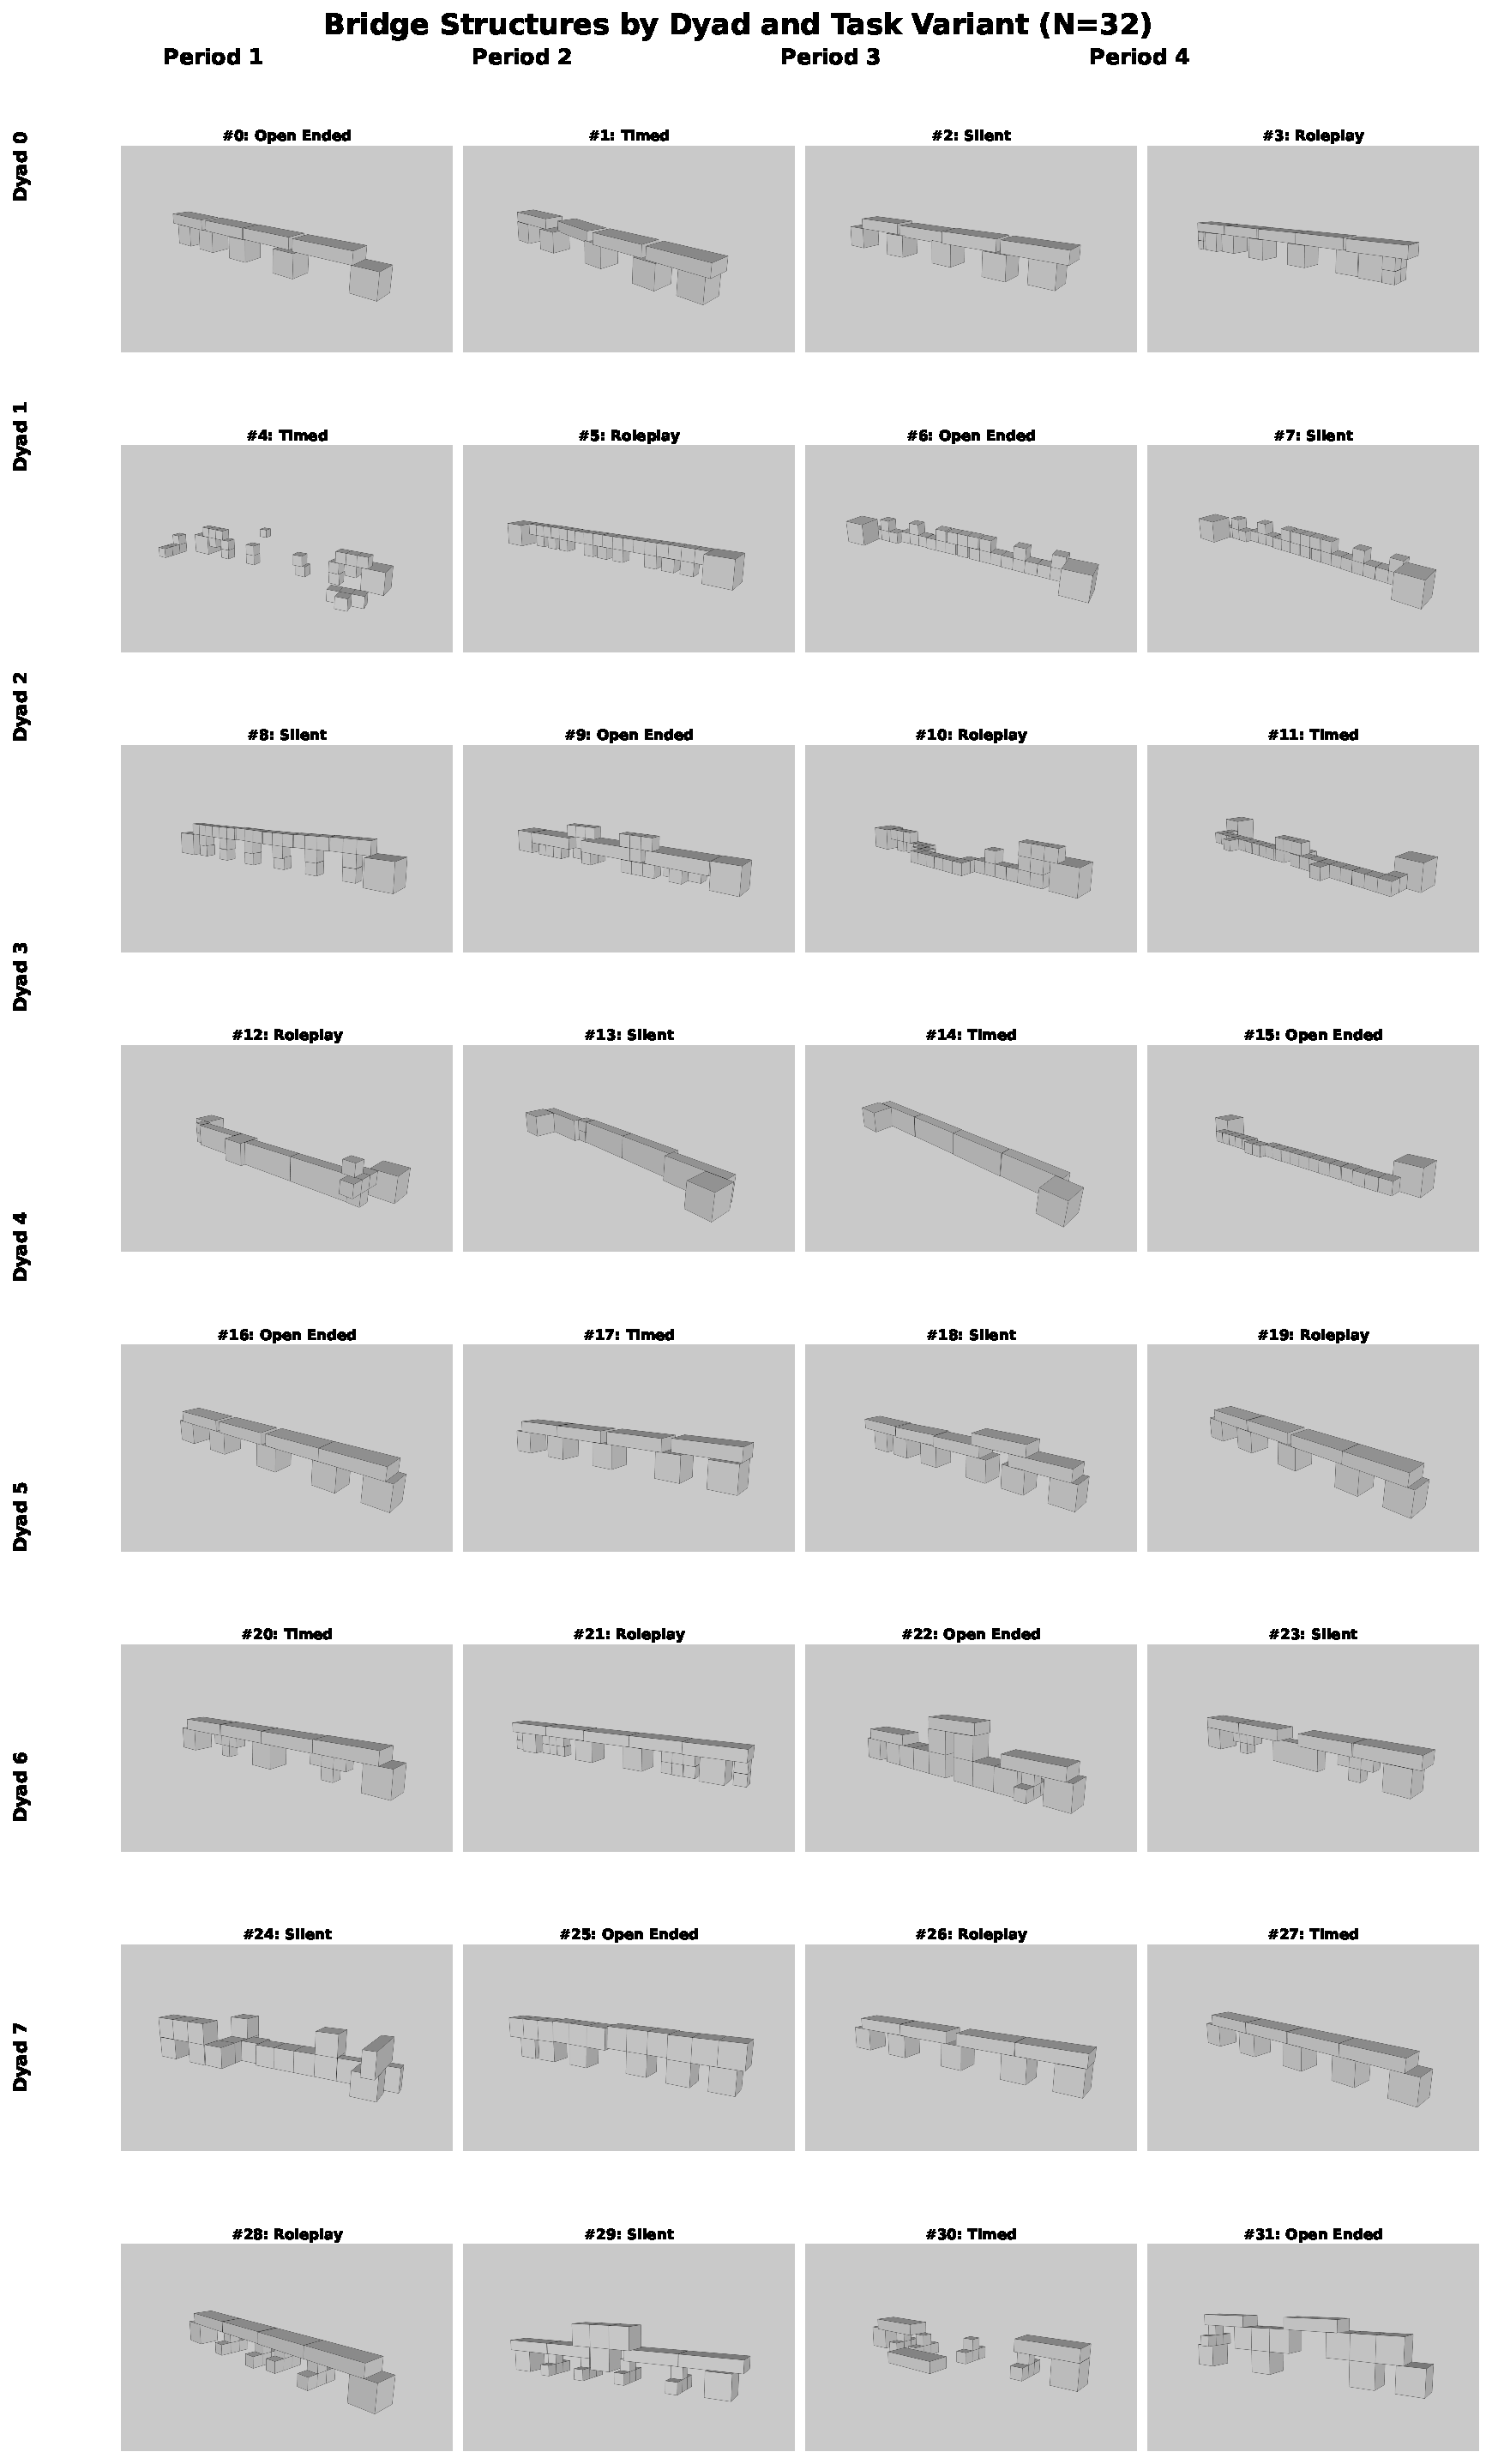
\includegraphics[width=\textwidth]{assets/06/bridge_structures_grid.pdf}
\caption{Complete overview of all 32 bridge structures organized by dyad and experimental period. Each dyad followed a different Latin square sequence, so columns represent different task variants for each row.}
\label{fig:bridge_structures_grid}
\end{figure}


\subsection{Complete Structural Analysis Data}
\begin{table}[H]
\centering
\caption{Bridge Quality Metrics - Complete Dataset (N=30 valid bridges)}
\label{tab:bridge_quality_complete}
\begin{tabular}{lrrrrrr}
\toprule
\textbf{Metric} & \textbf{N} & \textbf{Mean} & \textbf{SD} & \textbf{Median} & \textbf{Min} & \textbf{Max} \\
\midrule
Safety Factor & 30 & 10.36 & 5.01 & 13.05 & 0.49 & 15.00 \\
von Mises Stress (MPa) & 30 & 121.43 & 306.71 & 22.03 & 0.00 & 1212.00 \\
Displacement (mm) & 30 & 268,132.70 & 1,466,543.31 & 0.05 & 0.00 & 8,032,961.00 \\
Price (cost units) & 30 & 59.73 & 40.51 & 57.50 & 14.00 & 186.00 \\
Height (cm) & 30 & 30.33 & 9.28 & 30.00 & 10.00 & 50.00 \\
Total Objects & 30 & 10.17 & 3.39 & 9.00 & 6.00 & 21.00 \\
Different Object Types & 30 & 2.20 & 0.71 & 2.00 & 1.00 & 4.00 \\
\bottomrule
\end{tabular}
\end{table}

\begin{table}[H]
\centering
\caption{Bridge Quality by Collaboration Variant - Detailed Statistics}
\label{tab:bridge_quality_by_variant_complete}
\begin{tabular}{llrrrr}
\toprule
\textbf{Metric} & \textbf{Variant} & \textbf{N} & \textbf{Mean} & \textbf{SD} & \textbf{Median} \\
\midrule
\multirow{4}{*}{Safety Factor} & Open Ended & 8 & 10.95 & 5.30 & 13.56 \\
& Silent & 8 & 7.70 & 5.34 & 6.84 \\
& Timed & 6 & 10.51 & 4.92 & 10.64 \\
& Roleplay & 8 & 12.32 & 4.14 & 14.14 \\
\midrule
\multirow{4}{*}{von Mises Stress (MPa)} & Open Ended & 8 & 42.56 & 78.54 & 15.28 \\
& Silent & 8 & 229.11 & 416.64 & 37.72 \\
& Timed & 6 & 221.10 & 485.66 & 33.96 \\
& Roleplay & 8 & 17.86 & 19.00 & 15.81 \\
\midrule
\multirow{4}{*}{Displacement (mm)} & Open Ended & 8 & 1,377.02 & 3,894.66 & 0.05 \\
& Silent & 8 & 1,004,120.30 & 2,840,080.53 & 0.09 \\
& Timed & 6 & 0.28 & 0.38 & 0.15 \\
& Roleplay & 8 & 0.09 & 0.21 & 0.02 \\
\midrule
\multirow{4}{*}{Construction Cost} & Open Ended & 8 & 62.63 & 48.29 & 53.0 \\
& Silent & 8 & 71.75 & 55.21 & 67.0 \\
& Timed & 6 & 52.33 & 23.06 & 58.0 \\
& Roleplay & 8 & 50.38 & 26.79 & 54.5 \\
\bottomrule
\end{tabular}
\end{table}

\subsection{Quality-Performance Correlation Analysis}

\begin{table}[H]
\centering
\caption{Bridge Quality vs Performance Correlations}
\label{tab:quality_performance_correlations}
\begin{tabular}{lrrr}
\toprule
\textbf{Quality Metric} & \textbf{vs Completion Time} & \textbf{vs Total Objects} & \textbf{vs Efficiency} \\
\midrule
Safety Factor & r = 0.093 (p = 0.625) & r = 0.121 (p = 0.523) & r = 0.089 (p = 0.642) \\
von Mises Stress & r = -0.202 (p = 0.284) & r = -0.156 (p = 0.411) & r = -0.112 (p = 0.558) \\
Displacement & r = 0.017 (p = 0.929) & r = -0.089 (p = 0.642) & r = 0.045 (p = 0.814) \\
Construction Cost & r = 0.025 (p = 0.895) & r = 0.489 (p = 0.006**) & r = 0.156 (p = 0.411) \\
\bottomrule
\end{tabular}
\small
**p < 0.01
\end{table}

\begin{table}[H]
\centering
\caption{Statistical Tests for Bridge Quality by Variant}
\label{tab:bridge_quality_tests_complete}
\begin{tabular}{lrrrl}
\toprule
\textbf{Metric} & \textbf{$\chi^2$ (Friedman)} & \textbf{df} & \textbf{p-value} & \textbf{Kendall's W} \\
\midrule
Safety Factor & 4.062 & 3 & 0.255 & 0.226 (medium) \\
von Mises Stress & 3.200 & 3 & 0.362 & 0.178 (medium) \\
Displacement & 2.288 & 3 & 0.515 & 0.127 (medium) \\
Construction Cost & 3.120 & 3 & 0.373 & 0.173 (medium) \\
Total Objects & 2.062 & 3 & 0.560 & 0.115 (small) \\
Bridge Height & 1.875 & 3 & 0.599 & 0.104 (small) \\
\bottomrule
\end{tabular}
\end{table}

% ============================================================================
\section{Collaboration Dynamics - Detailed Results}  
\label{appendix:movement_results}
% ============================================================================

This section provides comprehensive analysis of movement patterns, spatial coordination, and collaboration dynamics across all task variants. The analysis includes partner synchronization metrics, statistical comparisons of movement efficiency, and relationships between movement patterns and task performance.

\subsection{Movement Patterns and Spatial Coordination}

This section presents the complete movement analysis including activity synchronization patterns between partners and statistical comparisons across task variants. Movement data was captured at 1Hz throughout all sessions and analyzed for coordination patterns, speed consistency, and individual differences.

\begin{table}[H]
\centering
\caption{Movement Analysis - Detailed Statistics by Variant}
\label{tab:movement_complete_stats}
\begin{tabular}{lrrrrr}
\toprule
\textbf{Variant} & \textbf{Avg Speed (m/min)} & \textbf{SD} & \textbf{Correlation (r)} & \textbf{p-value} & \textbf{Asymmetry} \\
\midrule
Open Ended & 20.75 & 8.69 & 0.890 & 0.003** & 0.22 \\
Silent & 23.02 & 8.83 & 0.351 & 0.394 & 0.24 \\
Timed & 29.38 & 12.51 & 0.939 & 0.001** & 0.18 \\
Roleplay & 22.29 & 13.68 & 0.658 & 0.076 & 0.71 \\
\midrule
\textbf{Overall} & 23.86 & 10.56 & 0.737 & < 0.001*** & 0.34 \\
\bottomrule
\end{tabular}
\small
*p < 0.05, **p < 0.01, ***p < 0.001
\end{table}

\begin{table}[H]
\centering
\caption{Individual Dyad Movement Synchronization Patterns}
\label{tab:dyad_movement_complete}
\begin{tabular}{lrrrrl}
\toprule
\textbf{Dyad} & \textbf{Correlation (r)} & \textbf{p-value} & \textbf{r²} & \textbf{Sessions} & \textbf{Coordination Level} \\
\midrule
SAKl2Kyg-jFYQhuSp & 0.996 & 0.004** & 0.992 & 4 & Near-perfect \\
kDp3Cy37-wocE408P & 0.988 & 0.012* & 0.976 & 4 & Near-perfect \\
OYYOwkG2-dckk6p6S & 0.984 & 0.016* & 0.968 & 4 & Very high \\
uTSV9lZx-iB6kR2uo & 0.945 & 0.055 & 0.893 & 4 & High \\
YeUp7E4D-WzyEiaaj & 0.753 & 0.247 & 0.567 & 4 & Moderate \\
Oa3Qww1v-zIDJJG4M & 0.718 & 0.282 & 0.516 & 4 & Moderate \\
6m7xtdFy-kHxWHBLy & 0.493 & 0.507 & 0.243 & 4 & Low \\
j7hHkgiC-iN9X5S4Q & 0.009 & 0.991 & 0.000 & 4 & Minimal \\
\bottomrule
\end{tabular}
\end{table}

\subsection{Statistical Tests for Movement Patterns}
\label{appendix:movement_communication}

This subsection provides the complete statistical test results for movement patterns, including Friedman tests for variant comparisons, correlation analyses for partner synchronization, and relationships between movement patterns and task performance.

\begin{table}[H]
\centering
\caption{Movement Pattern Statistical Analysis}
\label{tab:movement_tests_complete}
\begin{tabular}{lrrrl}
\toprule
\textbf{Analysis} & \textbf{Test Statistic} & \textbf{df} & \textbf{p-value} & \textbf{Effect/Interpretation} \\
\midrule
\textbf{Movement Efficiency by Variant} & $\chi^2 = 3.750$ & 3 & 0.290 & No significant differences \\
\textbf{Total Movement by Variant} & $\chi^2 = 7.875$ & 3 & 0.049* & Confounded by duration \\
\textbf{Partner Correlation Overall} & r = 0.737 & & < 0.001*** & Strong synchronization \\
\textbf{Movement vs Performance} & r = -0.332 & & 0.064 & Marginal negative correlation \\
\textbf{Learning Effect (Position)} & r = 0.071 & & 0.703 & No learning in movement \\
\bottomrule
\end{tabular}
\end{table}

% ============================================================================
\section{Communication Patterns - Detailed Results}
\label{appendix:communication_results}
% ============================================================================

This section presents detailed communication analysis including volume measures, turn-taking patterns, spatial language usage, and content categorization across the three verbal task variants (Open Ended, Timed, and Roleplay). The Silent condition is excluded from communication analysis by design.

\subsection{Complete Communication Analysis}

This section provides comprehensive communication analysis including word counts, turn patterns, spatial language usage, and correlations between communication measures and task performance. Analysis covers 24 sessions with verbal communication (Silent condition excluded by design).

\begin{table}[H]
\centering
\caption{Communication Patterns - Complete Statistics by Variant}
\label{tab:communication_complete_stats}
\begin{tabular}{lrrrrr}
\toprule
\textbf{Metric} & \textbf{Open Ended} & \textbf{Timed} & \textbf{Roleplay} & \textbf{Test Stat} & \textbf{p-value} \\
\midrule
Total Words (mean ± SD) & 472 ± 303 & 341 ± 303 & 1172 ± 1142 & $\chi^2 = 9.750$ & 0.008** \\
Words per Minute & 65.1 ± 30.9 & 69.8 ± 31.1 & 77.7 ± 36.1 & $\chi^2 = 0.750$ & 0.687 \\
Turns per Minute & 10.7 ± 4.1 & 9.8 ± 2.8 & 9.9 ± 3.3 & $\chi^2 = 2.250$ & 0.325 \\
Communication Balance & 0.39 ± 0.25 & 0.51 ± 0.36 & 0.33 ± 0.30 & $\chi^2 = 1.750$ & 0.417 \\
Deictic Density (\%) & 6.8 ± 1.4 & 6.1 ± 2.0 & 6.5 ± 1.8 & $\chi^2 = 0.250$ & 0.882 \\
Spatial Density (\%) & 2.0 ± 0.8 & 2.0 ± 0.9 & 2.0 ± 0.4 & $\chi^2 = 2.250$ & 0.325 \\
Planning Ratio (\%) & 31.7 ± 12.1 & 32.6 ± 8.2 & 32.1 ± 11.0 & $\chi^2 = 0.750$ & 0.687 \\
Turn Transitions & 22.1 ± 14.2 & 10.9 ± 9.5 & 40.6 ± 38.3 & $\chi^2 = 8.968$ & 0.011* \\
\bottomrule
\end{tabular}
\small
*p < 0.05, **p < 0.01
\end{table}

\begin{table}[H]
\centering
\caption{Communication Volume and Performance Relationships}
\label{tab:communication_performance_complete}
\begin{tabular}{lrrr}
\toprule
\textbf{Relationship} & \textbf{Correlation (r)} & \textbf{p-value} & \textbf{Interpretation} \\
\midrule
Total Words vs Completion Time & 0.523 & 0.009** & Positive (expected) \\
Words per Minute vs Completion Time & 0.034 & 0.873 & No relationship \\
Communication Balance vs Performance & -0.187 & 0.383 & Weak negative \\
Deictic Density vs Task Efficiency & 0.156 & 0.467 & Weak positive \\
Planning Ratio vs Bridge Quality & 0.089 & 0.678 & No relationship \\
\bottomrule
\end{tabular}
\end{table}

% ============================================================================
\section{System Performance and Subjective Experience}
\label{appendix:results:subjective}
% ============================================================================

\subsection{System Usability and Workload Progression}
\label{appendix:subjective}

\begin{table}[H]
\centering
\caption{System Usability Scale (SUS) and NASA-TLX by Session}
\label{tab:sus_tlx_complete}
\begin{tabular}{lrrrrrrr}
\toprule
\textbf{Session} & \textbf{SUS Mean} & \textbf{SUS SD} & \textbf{SUS SE} & \textbf{TLX Mean} & \textbf{TLX SD} & \textbf{TLX SE} & \textbf{N} \\
\midrule
1 & 67.5 & 11.1 & 2.8 & 7.3 & 10.8 & 2.7 & 16 \\
2 & 70.6 & 14.0 & 3.5 & 18.0 & 18.2 & 4.5 & 16 \\
3 & 69.8 & 15.4 & 3.8 & 18.0 & 23.8 & 6.0 & 16 \\
4 & 72.5 & 13.8 & 3.5 & 9.7 & 13.7 & 3.4 & 16 \\
\midrule
\textbf{Change (1→4)} & \textbf{+5.0*} & & & \textbf{+2.5} & & & \\
\textbf{Effect Size} & \textbf{d = 0.98} & & & \textbf{d = 0.19} & & & \\
\bottomrule
\end{tabular}
\small
*p < 0.05 (t = 2.760, p = 0.015)
\end{table}

\begin{table}[H]
\centering
\caption{Learning Effects by AR/VR Experience Level}
\label{tab:experience_learning_complete}
\begin{tabular}{lrrrrrr}
\toprule
\textbf{Experience} & \textbf{N} & \textbf{Initial SUS} & \textbf{Final SUS} & \textbf{Change} & \textbf{Completion Time} & \textbf{Performance} \\
\midrule
None & 3 & 67.5 ± 8.8 & 72.5 ± 6.6 & +5.0 & 7.28 ± 3.12 & Baseline \\
Limited & 6 & 64.2 ± 11.8 & 73.8 ± 15.6 & +9.6 & 7.85 ± 2.89 & Similar \\
Moderate & 5 & 72.5 ± 10.4 & 71.5 ± 15.1 & -1.0 & 8.48 ± 3.21 & Slowest \\
Extensive & 2 & 81.3 ± 12.4 & 87.5 ± 3.5 & +6.2 & 6.41 ± 2.15 & Fastest \\
\bottomrule
\end{tabular}
\end{table}

\subsection{Relationship and Trust Measures}

\begin{table}[H]
\centering
\caption{Interpersonal Relationship Measures Pre-Post Study}
\label{tab:relationship_measures_complete}
\begin{tabular}{lrrrrl}
\toprule
\textbf{Measure} & \textbf{Pre-Study} & \textbf{Post-Study} & \textbf{Change} & \textbf{p-value} & \textbf{Effect} \\
\midrule
IOS (Inclusion of Other in Self) & 3.69 ± 1.25 & 3.75 ± 1.18 & +0.06 & 0.789 & No change \\
Partner Competence Rating & 4.2 ± 0.8 & 4.3 ± 0.7 & +0.1 & 0.678 & No change \\
Collaboration Satisfaction & N/A & 4.1 ± 0.9 & N/A & N/A & High satisfaction \\
\bottomrule
\end{tabular}
\end{table}

% ============================================================================
\section{Individual Differences and Personality Effects}
\label{appendix:individual_differences}
% ============================================================================

\begin{table}[H]
\centering
\caption{Personality-Performance Correlation Matrix}
\label{tab:personality_complete}
\begin{tabular}{lrrrrr}
\toprule
\textbf{Big Five Trait} & \textbf{Completion Time} & \textbf{Bridge Quality} & \textbf{SUS Score} & \textbf{Movement Sync} & \textbf{Communication} \\
\midrule
Openness & -0.409 (0.115) & 0.122 (0.657) & 0.234 (0.386) & 0.067 (0.805) & 0.156 (0.572) \\
Conscientiousness & -0.009 (0.974) & 0.089 (0.741) & 0.156 (0.563) & -0.234 (0.386) & -0.089 (0.741) \\
Extraversion & -0.111 (0.682) & -0.034 (0.900) & 0.301 (0.256) & 0.178 (0.512) & 0.234 (0.386) \\
Agreeableness & -0.036 (0.895) & 0.201 (0.456) & 0.189 (0.483) & 0.089 (0.741) & -0.067 (0.805) \\
Neuroticism & -0.116 (0.668) & -0.156 (0.563) & -0.223 (0.408) & -0.112 (0.682) & 0.023 (0.932) \\
\bottomrule
\end{tabular}
\small
Values shown as r (p-value). No correlations reach statistical significance.
\end{table}

\begin{table}[H]
\centering
\caption{Demographic Effects on Performance}
\label{tab:demographics_performance_complete}
\begin{tabular}{lrrrrr}
\toprule
\textbf{Factor} & \textbf{N} & \textbf{Completion Time} & \textbf{Bridge Quality} & \textbf{SUS Progression} & \textbf{Notes} \\
\midrule
\textbf{Gender} & & & & & \\
Male & 10 & 7.59 ± 2.83 & 10.2 ± 4.8 & +4.8 & Similar performance \\
Female & 6 & 7.89 ± 3.50 & 10.6 ± 5.4 & +5.3 & Similar performance \\
\midrule
\textbf{Age Correlation} & 16 & r = 0.424 (0.101) & r = -0.156 (0.563) & r = -0.089 (0.741) & Marginal age effect \\
\midrule
\textbf{Language} & & & & & \\
German & 13 & 7.68 ± 2.94 & 10.5 ± 4.9 & +5.2 & Majority group \\
Other & 3 & 7.93 ± 4.11 & 9.8 ± 5.8 & +4.0 & Small sample \\
\bottomrule
\end{tabular}
\end{table}

% ============================================================================
\section{Construction Efficiency and Material Usage}
\label{appendix:construction}
% ============================================================================

\begin{table}[H]
\centering
\caption{Construction Efficiency and Resource Usage by Variant}
\label{tab:construction_complete}
\begin{tabular}{lrrrrrr}
\toprule
\textbf{Variant} & \textbf{Objects Used} & \textbf{Objects Spawned} & \textbf{Efficiency} & \textbf{Waste \%} & \textbf{Types Used} & \textbf{N} \\
\midrule
Open Ended & 10.1 ± 3.2 & 22.2 ± 8.1 & 0.478 ± 0.113 & 52.2 & 2.38 ± 0.74 & 8 \\
Silent & 10.0 ± 2.8 & 19.0 ± 7.2 & 0.638 ± 0.323 & 36.2 & 2.00 ± 0.53 & 8 \\
Timed & 8.5 ± 2.1 & 11.7 ± 4.3 & 0.810 ± 0.335 & 19.0 & 2.00 ± 0.63 & 6 \\
Roleplay & 11.6 ± 4.1 & 26.2 ± 9.8 & 0.524 ± 0.259 & 47.6 & 2.71 ± 0.95 & 8 \\
\bottomrule
\end{tabular}
\end{table}

\begin{table}[H]
\centering
\caption{Building Block Type Preferences by Variant (\% of spawned objects)}
\label{tab:block_preferences_complete}
\begin{tabular}{lrrrr}
\toprule
\textbf{Block Type} & \textbf{Open Ended} & \textbf{Silent} & \textbf{Timed} & \textbf{Roleplay} \\
\midrule
BigTShape & 12.4 & 4.6 & 1.4 & 1.0 \\
Cube & 9.6 & 11.8 & 24.3 & 21.0 \\
Plank & 19.1 & 35.5 & 48.6 & 28.1 \\
SmallCube & 27.5 & 13.8 & 1.4 & 27.6 \\
BigLShape & 6.7 & 2.0 & 1.4 & 0.0 \\
TShape & 20.2 & 32.2 & 2.9 & 17.1 \\
LShape & 4.5 & 0.0 & 20.0 & 5.2 \\
\bottomrule
\end{tabular}
\end{table}

% ============================================================================
\section{Statistical Power Analysis and Effect Sizes}
\label{appendix:power_analysis}
% ============================================================================

\begin{table}[H]
\centering
\caption{Power Analysis Results for Key Statistical Tests}
\label{tab:power_analysis_complete}
\begin{tabular}{lrrrl}
\toprule
\textbf{Test Type} & \textbf{Sample Size} & \textbf{Observed Power} & \textbf{Effect Size} & \textbf{Interpretation} \\
\midrule
\textbf{Friedman Test (n=8 dyads, 4 conditions)} & & & & \\
Small effects (f = 0.25) & 8 & 0.14 & Kendall's W = 0.14 & Underpowered \\
Medium effects (f = 0.40) & 8 & 0.34 & Kendall's W = 0.34 & Underpowered \\
Large effects (f = 0.60) & 8 & 0.71 & Kendall's W = 0.53 & Adequate for large effects \\
\midrule
\textbf{Wilcoxon Signed-Rank (n=8 pairs)} & & & & \\
Medium effects (d = 0.5) & 8 & 0.19 & r = 0.46 & Underpowered \\
Large effects (d = 0.8) & 8 & 0.43 & r = 0.80 & Marginal power \\
Very large effects (d = 1.3) & 8 & 0.80 & r = 0.94 & Adequate power \\
\midrule
\textbf{Correlation Analysis (n=16 individuals)} & & & & \\
Medium correlations (r = 0.5) & 16 & 0.51 & & Underpowered \\
Large correlations (r = 0.7) & 16 & 0.88 & & Adequate power \\
\bottomrule
\end{tabular}
\end{table}

% ============================================================================
% \section{Key Statistical Results Summary}
% \label{appendix:stats_summary}
% % ============================================================================

% \subsection{Significant Effects (p < 0.05)}
% \begin{itemize}
% \item \textbf{Collaboration variant on completion time}: Friedman $\chi^2$ = 12.750, p = 0.005, Kendall's W = 0.531 (large effect)
% \item \textbf{Silent vs verbal communication}: Mann-Whitney U = 27.0, p = 0.025, r = 0.46 (medium effect)
% \item \textbf{Roleplay vs other variants}: Multiple comparisons p < 0.05, large effect sizes (r > 0.8)
% \item \textbf{Total communication volume by variant}: Friedman $\chi^2$ = 9.750, p = 0.008
% \item \textbf{Turn transitions by variant}: Friedman $\chi^2$ = 8.968, p = 0.011
% \item \textbf{Movement synchronization overall}: r = 0.737, p < 0.001 (large effect)
% \item \textbf{SUS learning effect}: t = 2.760, p = 0.015, Cohen's d = 0.98 (large effect)
% \end{itemize}

% \subsection{Non-significant Effects (p > 0.05)}
% \begin{itemize}
% \item Virtual environment on any performance metric (p = 0.522)
% \item Task position (learning) on completion time overall (p = 0.440)
% \item Bridge quality metrics by collaboration variant (all p > 0.25)
% \item Personality traits on task performance (all p > 0.10)
% \item NASA-TLX workload changes across sessions (p = 0.597)
% \item Movement efficiency by variant (p = 0.290)
% \item Communication density and spatial reference patterns by variant
% \end{itemize}

% \subsection{Effect Sizes and Practical Significance}
% \begin{itemize}
% \item \textbf{Communication paradox}: Silent condition 2.2× faster than verbal conditions
% \item \textbf{Time pressure effect}: Timed variant 3.1× faster than untimed variants
% \item \textbf{Role conflict overhead}: Roleplay variant 2.6× slower with 2.2× more movement
% \item \textbf{Movement synchronization}: Strongest effect in study (r = 0.737, large effect)
% \item \textbf{Quality-speed independence}: No meaningful correlations across all quality measures
% \item \textbf{Learning effect}: 5-point SUS improvement with large effect size (d = 0.98)
% \end{itemize}

% \subsection{Interpretive Notes}
% Given the study's power limitations, non-significant findings with small-to-medium effect sizes should be considered \textbf{inconclusive} rather than evidence of no effect. The significant effects observed represent genuinely substantial differences that exceeded the study's detection threshold. All effect size interpretations follow Cohen's conventions: small (0.2), medium (0.5), large (0.8) for d; small (0.1), medium (0.3), large (0.5) for r.

\section{Communication Coding Categories}\label{appendix:coding_categories}

This section documents the specific word lists and coding schemes used for transcript analysis presented in Section~\ref{sec:communication}. All word matching was performed using case-insensitive regular expressions on participant utterances (statements by host excluded).

\subsection{Spatial Reference Coding}

Spatial references were identified using two main categories: deictic references and directional/positional language.

\subsubsection{Deictic Reference Patterns}
Basic spatial deixis patterns using regular expressions:
\begin{itemize}
\item \texttt{\\b(here|there|this|that)\\b} - Basic spatial demonstratives
\item \texttt{\\b(left|right|up|down|over|under)\\b} - Directional terms
\item \texttt{\\b(next to|beside|behind|in front)\\b} - Relational positioning
\item \texttt{\\b(put|place|move|go)\\s+(it|this|that|there|here)\\b} - Action-location combinations
\item \texttt{\\b(on|in|at|to|from)\\s+(the|this|that)\\b} - Prepositional references
\end{itemize}

\subsubsection{Calculation Method}
Spatial reference density was calculated as:
$$\text{Spatial Density} = \frac{\text{Total Spatial References}}{\text{Total Words in Session}}$$

This metric represents the proportion of words dedicated to spatial coordination language.

\subsection{Planning vs. Execution Communication}

Communication was categorized into planning-oriented and execution-oriented language based on distinct word patterns.

\subsubsection{Planning Language Patterns}
Planning-related communication included three subcategories:

\textbf{Strategy and Deliberation:}
\begin{itemize}
\item \texttt{plan}, \texttt{strategy}, \texttt{should}, \texttt{let's}, \texttt{how about}, \texttt{what if}, \texttt{we could}
\end{itemize}

\textbf{Temporal Sequencing:}
\begin{itemize}
\item \texttt{first}, \texttt{then}, \texttt{next}, \texttt{after}, \texttt{before}
\end{itemize}

\textbf{Ideation and Reflection:}
\begin{itemize}
\item \texttt{idea}, \texttt{think}, \texttt{suggest}, \texttt{propose}
\end{itemize}

\subsubsection{Execution Language Patterns}
Execution-related communication included three subcategories:

\textbf{Direct Actions:}
\begin{itemize}
\item \texttt{put}, \texttt{place}, \texttt{move}, \texttt{grab}, \texttt{take}, \texttt{drop}
\end{itemize}

\textbf{Immediate Coordination:}
\begin{itemize}
\item \texttt{there}, \texttt{here}, \texttt{now}, \texttt{wait}, \texttt{good}, \texttt{done}
\end{itemize}

\textbf{Confirmation and Response:}
\begin{itemize}
\item \texttt{yes}, \texttt{no}, \texttt{ok}, \texttt{okay}, \texttt{right}, \texttt{wrong}
\end{itemize}

\subsubsection{Calculation Method}
Planning ratio was calculated as:
$$\text{Planning Ratio} = \frac{\text{Planning Utterances}}{\text{Planning Utterances + Execution Utterances}}$$

Only utterances containing planning or execution markers were included in this ratio calculation.

\subsection{Content Theme Analysis}

Additional thematic content analysis used the following categories:

\textbf{Building Actions:}
\begin{itemize}
\item \texttt{build}, \texttt{place}, \texttt{put}, \texttt{move}, \texttt{position}, \texttt{block}, \texttt{cube}, \texttt{plank}
\end{itemize}

\textbf{Planning and Strategy:}
\begin{itemize}
\item \texttt{plan}, \texttt{strategy}, \texttt{idea}, \texttt{think}, \texttt{should}, \texttt{could}, \texttt{would}, \texttt{maybe}
\end{itemize}

\textbf{Spatial Coordination:}
\begin{itemize}
\item \texttt{here}, \texttt{there}, \texttt{this}, \texttt{that}, \texttt{left}, \texttt{right}, \texttt{side}, \texttt{middle}
\end{itemize}

\textbf{Evaluation and Quality:}
\begin{itemize}
\item \texttt{good}, \texttt{bad}, \texttt{better}, \texttt{worse}, \texttt{price}, \texttt{cost}, \texttt{strong}, \texttt{stable}
\end{itemize}

\textbf{Problem Identification:}
\begin{itemize}
\item \texttt{problem}, \texttt{issue}, \texttt{wrong}, \texttt{error}, \texttt{stuck}, \texttt{difficult}, \texttt{help}
\end{itemize}

\textbf{Agreement and Acknowledgment:}
\begin{itemize}
\item \texttt{yes}, \texttt{okay}, \texttt{right}, \texttt{sure}, \texttt{agree}, \texttt{no}, \texttt{wait}
\end{itemize}

\subsection{Implementation Details}

All coding was implemented using Python regular expressions with the following considerations:
\begin{itemize}
\item Word boundary matching (\texttt{\\b}) to avoid partial word matches
\item Case-insensitive matching for consistent results
\item Substring matching for morphological variations (e.g., "building" matches "build")
\item Exclusion of HOST utterances from all participant communication metrics
\end{itemize}

The analysis scripts are available in the \texttt{user-study-analysis/} directory, with primary implementations in \texttt{transcript\_analysis.py} and \texttt{communication\_analysis.py}.
